\chapter{Literature review}\label{chapter:gamification}


\section{Gamification}

In recent years, there have been an tremendous increase in popularity of video games inspired software solutions (cite maybe) which main goals are to develop new skills, solve problems or address issues in a variety of functional areas. TO ADD EXAMPLES What these software solutions all have in common is that they are based on the concept of \textit{gamification}, defined by Detering \textit{et al} (2011) as ``the use of game design elements in a non-game context''  \cite{deterding2011game}. In parallel with this term, a verb \textit{to gamify} has been defined. It's meaning reffers to applying game mechanics to supercharge user engagement, loyalty and fun \cite{toGamify}. It should be noted that the definition of gamification outlined by Detering \textit{et al.} relates to \textit{games} and not \textit{play} \cite{deterding2011game}. Even though often used interchangeably, there exists a complex relationship between these two concept and clear distinction can be made. That is, according to the forms they take in the world, \textit{play} can be interpreted as a broader category that includes \textit{game} as a subset \cite{salen2004rules}. 
Game design elements represent parts of games used as a building block for creating gamified applications. They are tools and rules that define the overall context of game \cite{gamDesElem}. This means that the definition distinguishes gamification from other systems that employ full-fledged games rather than elements of game design only. Furthermore, it does not include all game elements either, only a subcategory called game design elements. %ova dve poslednje recenice odavde, izmeni 
%http://ludus.hu/en/gamification/
Game design elements are themselves difficult to specify and often are described on varying levels of abstraction. Derived from the available literature, Deterding et al. found that previously identified game elements fell into five distinct levels of abstraction. Table \ref{table:gameElements} lists the five levels of game elements, ordered from concrete to abstract.
% Please add the following required packages to your document preamble:
% \usepackage{booktabs}
% \usepackage{graphicx}
% \usepackage[normalem]{ulem}
% \useunder{\uline}{\ul}{}
\begin{table}[]
\centering
\caption{Taxonomy of game design elements by level of abstraction}
\label{table:gameElements}
\resizebox{\textwidth}{!}{%
\begin{tabular}{@{}lll@{}}
\toprule
\textbf{Level} & \textbf{Description} & \textbf{Example} \\ \midrule
\begin{tabular}[c]{@{}l@{}}Game interface\\ design patterns\end{tabular} & \begin{tabular}[c]{@{}l@{}}Common, successful interaction design components and design solutions for\\ a known problem in a context, including prototypical implementations\end{tabular} & Badge, leaderboard, level \\
\begin{tabular}[c]{@{}l@{}}Game design\\ patterns and\\ mechanics\end{tabular} & Commonly reoccurring parts of the design of a game that concern gameplay & Time constraint, limited resources, turns \\
\begin{tabular}[c]{@{}l@{}}Game design\\ principles and\\ heuristics\end{tabular} & \begin{tabular}[c]{@{}l@{}}Evaluative guidelines to approach a design problem or analyze a given\\ design solution\end{tabular} & Enduring play, clear goals, variety of game styles \\
Game models & Conceptual models of the components of games or game experience & \begin{tabular}[c]{@{}l@{}}Mechanics–Dynamics–Esthetics (MDA); challenge, fantasy, curiosity;\\ game design atoms; Core Elements of the Gaming Experience (CEGE)\end{tabular} \\
\begin{tabular}[c]{@{}l@{}}Game design\\ methods\end{tabular} & Game design-specific practices and processes & Playtesting, playcentric design, value conscious game design \\ \bottomrule
\end{tabular}%
}
\end{table}
%With respect to the use of game design elements, gamification studies classified gamification elements differently \cite{schobel2016agony}.% Sch{\"o}bel \textit{et al.} carried out a literature review to analyze the gamification elements used in various research studies.
%prezentacija o game vs play http://gamification-research.org/2012/04/defining-gamification/
%detering definise elements of game design. five leveles.
Lastly, a non-game contexts refers to applications which main purpose is beyond pure entertainment and wher gamification has been applied (i.e. business, personal improvement, education, health, etc.)
\cite{deterding2011situated}
The definition of gamification is closely related to similar pre-existing concepts such as serious games and playful interaction \cite{deterding2011game}. However, the concept of gamification can be differentiated from these similar phenomena on a two-by-two matrix introduced by Detering \textit{et al.}(figure \ref{fig:mesh1}). 

\begin{figure}[h]
    \centering
    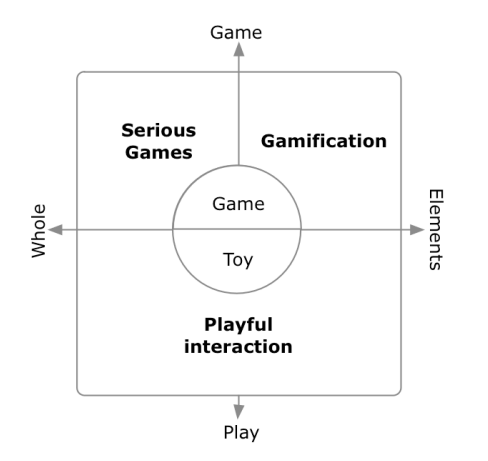
\includegraphics[width=0.50\textwidth]{gamification-btw-game-and-play2}
    \caption{The matrix distinguishing the concepts related to gamification}
    \label{fig:mesh1}
\end{figure}
 
In figure \ref{fig:mesh1}, along one axis Detering \textit{et al.} a distinction between gaming and playing is made, and on the other between whole or partial artefacts. They place gamification or gameful design in the quadrant involving games and partial artefacts, meaning that gamification uses gameful design rather than playful design and game elements rather than full-fledged games. 
 highlights the differences between gamification, serious games (games
for non-entertainment purposes) and playful interaction. Gamification is about
elements of games, not of play.26 Play is normally assumed to be a free-form
activity devoid of constraints whereas games are limited in action by rules and
provide context for actions.27 
 
 
%% add gamification example reference
% 

In theory, any context, task or process can be gamified \cite{muntean2011raising}. %skini i procitaj Muntean!! 

The main goal of gamification is to engage the users 
Gamification’s main goal is to rise the engagement of users by using game-like techniques such as
scoreboards and personalized fast feedback (Flatla et al, 2011) making people feel more ownership
and purpose when engaging with tasks (Pavlus, 2010). 
\cite{burke2016gamify}

Figure 1: 
Gamification in Health and Fitness has rapidly emerged over the past decade as a tool to promote health and wellness. It is a broad term referring to the use of game thinking and game mechanics in a non-game context to engage users and solve problems. The concept is used to incentivise users to achieve their goals and increase user engagement. The best examples of gamification are in the Health and Fitness industry, where games encourage exercise by turning physical activity into a game and by delivering health interventions for bad habits cessation, like smoking, overeating or poor hydration, and medication adherence. Application of mobile and wearable devices have proven to be effective platforms for health and fitness games due to its wide adaptation, ease of use and continuous proximity to the users and patients.



Since gamification can be applied to almost any business model, serious or not,
for this thesis, we restrict our concern of gamification to the solving of serious issues. In
particular, we are focused on gamification of education and behavior change related to the
serious world issue of childhood obesity